% Options for packages loaded elsewhere
% Options for packages loaded elsewhere
\PassOptionsToPackage{unicode}{hyperref}
\PassOptionsToPackage{hyphens}{url}
\PassOptionsToPackage{dvipsnames,svgnames,x11names}{xcolor}
%
\documentclass[
]{agujournal2019}
\usepackage{xcolor}
\usepackage{amsmath,amssymb}
\setcounter{secnumdepth}{5}
\usepackage{iftex}
\ifPDFTeX
  \usepackage[T1]{fontenc}
  \usepackage[utf8]{inputenc}
  \usepackage{textcomp} % provide euro and other symbols
\else % if luatex or xetex
  \usepackage{unicode-math} % this also loads fontspec
  \defaultfontfeatures{Scale=MatchLowercase}
  \defaultfontfeatures[\rmfamily]{Ligatures=TeX,Scale=1}
\fi
\usepackage{lmodern}
\ifPDFTeX\else
  % xetex/luatex font selection
\fi
% Use upquote if available, for straight quotes in verbatim environments
\IfFileExists{upquote.sty}{\usepackage{upquote}}{}
\IfFileExists{microtype.sty}{% use microtype if available
  \usepackage[]{microtype}
  \UseMicrotypeSet[protrusion]{basicmath} % disable protrusion for tt fonts
}{}
\makeatletter
\@ifundefined{KOMAClassName}{% if non-KOMA class
  \IfFileExists{parskip.sty}{%
    \usepackage{parskip}
  }{% else
    \setlength{\parindent}{0pt}
    \setlength{\parskip}{6pt plus 2pt minus 1pt}}
}{% if KOMA class
  \KOMAoptions{parskip=half}}
\makeatother
% Make \paragraph and \subparagraph free-standing
\makeatletter
\ifx\paragraph\undefined\else
  \let\oldparagraph\paragraph
  \renewcommand{\paragraph}{
    \@ifstar
      \xxxParagraphStar
      \xxxParagraphNoStar
  }
  \newcommand{\xxxParagraphStar}[1]{\oldparagraph*{#1}\mbox{}}
  \newcommand{\xxxParagraphNoStar}[1]{\oldparagraph{#1}\mbox{}}
\fi
\ifx\subparagraph\undefined\else
  \let\oldsubparagraph\subparagraph
  \renewcommand{\subparagraph}{
    \@ifstar
      \xxxSubParagraphStar
      \xxxSubParagraphNoStar
  }
  \newcommand{\xxxSubParagraphStar}[1]{\oldsubparagraph*{#1}\mbox{}}
  \newcommand{\xxxSubParagraphNoStar}[1]{\oldsubparagraph{#1}\mbox{}}
\fi
\makeatother


\usepackage{longtable,booktabs,array}
\usepackage{calc} % for calculating minipage widths
% Correct order of tables after \paragraph or \subparagraph
\usepackage{etoolbox}
\makeatletter
\patchcmd\longtable{\par}{\if@noskipsec\mbox{}\fi\par}{}{}
\makeatother
% Allow footnotes in longtable head/foot
\IfFileExists{footnotehyper.sty}{\usepackage{footnotehyper}}{\usepackage{footnote}}
\makesavenoteenv{longtable}
\usepackage{graphicx}
\makeatletter
\newsavebox\pandoc@box
\newcommand*\pandocbounded[1]{% scales image to fit in text height/width
  \sbox\pandoc@box{#1}%
  \Gscale@div\@tempa{\textheight}{\dimexpr\ht\pandoc@box+\dp\pandoc@box\relax}%
  \Gscale@div\@tempb{\linewidth}{\wd\pandoc@box}%
  \ifdim\@tempb\p@<\@tempa\p@\let\@tempa\@tempb\fi% select the smaller of both
  \ifdim\@tempa\p@<\p@\scalebox{\@tempa}{\usebox\pandoc@box}%
  \else\usebox{\pandoc@box}%
  \fi%
}
% Set default figure placement to htbp
\def\fps@figure{htbp}
\makeatother


% definitions for citeproc citations
\NewDocumentCommand\citeproctext{}{}
\NewDocumentCommand\citeproc{mm}{%
  \begingroup\def\citeproctext{#2}\cite{#1}\endgroup}
\makeatletter
 % allow citations to break across lines
 \let\@cite@ofmt\@firstofone
 % avoid brackets around text for \cite:
 \def\@biblabel#1{}
 \def\@cite#1#2{{#1\if@tempswa , #2\fi}}
\makeatother
\newlength{\cslhangindent}
\setlength{\cslhangindent}{1.5em}
\newlength{\csllabelwidth}
\setlength{\csllabelwidth}{3em}
\newenvironment{CSLReferences}[2] % #1 hanging-indent, #2 entry-spacing
 {\begin{list}{}{%
  \setlength{\itemindent}{0pt}
  \setlength{\leftmargin}{0pt}
  \setlength{\parsep}{0pt}
  % turn on hanging indent if param 1 is 1
  \ifodd #1
   \setlength{\leftmargin}{\cslhangindent}
   \setlength{\itemindent}{-1\cslhangindent}
  \fi
  % set entry spacing
  \setlength{\itemsep}{#2\baselineskip}}}
 {\end{list}}
\usepackage{calc}
\newcommand{\CSLBlock}[1]{\hfill\break\parbox[t]{\linewidth}{\strut\ignorespaces#1\strut}}
\newcommand{\CSLLeftMargin}[1]{\parbox[t]{\csllabelwidth}{\strut#1\strut}}
\newcommand{\CSLRightInline}[1]{\parbox[t]{\linewidth - \csllabelwidth}{\strut#1\strut}}
\newcommand{\CSLIndent}[1]{\hspace{\cslhangindent}#1}



\setlength{\emergencystretch}{3em} % prevent overfull lines

\providecommand{\tightlist}{%
  \setlength{\itemsep}{0pt}\setlength{\parskip}{0pt}}



 


\usepackage{url} %this package should fix any errors with URLs in refs.
\usepackage{lineno}
\usepackage[inline]{trackchanges} %for better track changes. finalnew option will compile document with changes incorporated.
\usepackage{soul}
\linenumbers
\makeatletter
\@ifpackageloaded{caption}{}{\usepackage{caption}}
\AtBeginDocument{%
\ifdefined\contentsname
  \renewcommand*\contentsname{Table of contents}
\else
  \newcommand\contentsname{Table of contents}
\fi
\ifdefined\listfigurename
  \renewcommand*\listfigurename{List of Figures}
\else
  \newcommand\listfigurename{List of Figures}
\fi
\ifdefined\listtablename
  \renewcommand*\listtablename{List of Tables}
\else
  \newcommand\listtablename{List of Tables}
\fi
\ifdefined\figurename
  \renewcommand*\figurename{Figure}
\else
  \newcommand\figurename{Figure}
\fi
\ifdefined\tablename
  \renewcommand*\tablename{Table}
\else
  \newcommand\tablename{Table}
\fi
}
\@ifpackageloaded{float}{}{\usepackage{float}}
\floatstyle{ruled}
\@ifundefined{c@chapter}{\newfloat{codelisting}{h}{lop}}{\newfloat{codelisting}{h}{lop}[chapter]}
\floatname{codelisting}{Listing}
\newcommand*\listoflistings{\listof{codelisting}{List of Listings}}
\makeatother
\makeatletter
\makeatother
\makeatletter
\@ifpackageloaded{caption}{}{\usepackage{caption}}
\@ifpackageloaded{subcaption}{}{\usepackage{subcaption}}
\makeatother
\usepackage{bookmark}
\IfFileExists{xurl.sty}{\usepackage{xurl}}{} % add URL line breaks if available
\urlstyle{same}
\hypersetup{
  pdftitle={Causal Inference of Labor Market Inequality Using PGM: A multidimensional analysis of unemployment rate and durations},
  pdfauthor={Mengjia Wei},
  pdfkeywords={PGM, Unemployment Rate, Unemployment Durations, Causal
Inference},
  colorlinks=true,
  linkcolor={blue},
  filecolor={Maroon},
  citecolor={Blue},
  urlcolor={Blue},
  pdfcreator={LaTeX via pandoc}}


\journalname{Georgetown Univeristy DSAN 5650 Journal}

\draftfalse

\begin{document}
\title{Causal Inference of Labor Market Inequality Using PGM: A
multidimensional analysis of unemployment rate and durations}

\authors{Mengjia Wei\affil{1}}
\affiliation{1}{Georgetown University, }



\begin{abstract}
In its revised report released on July 31, 2025, the U.S. Bureau of
Labor Statistics (BLS) reported a sharp slowdown in job creation
beginning in May, signaling heightened uncertainty and growing concerns
about the overall health of the U.S. labor market. This study
investigates the causal relationships between race, industry and
unemployment rates in the United States, applying~probabilistic
graphical modeling (PGM)~to uncover latent dependency structures across
demographic and industry variables. Using a PGM framework, we extend
this approach to labor market data by constructing conditional
dependence networks across two key dimensions: group attributes (race
and industry) and time (2024 vs.~2025). Specifically, the study examines
recent college graduates (ages 22--24) relative to older individuals
(25+), comparing their unemployment rates across 2024 and 2025. This
study first examined the race effect on the unemployment rate disparitu.
The industry-specific unemployment rate dynamics focuses on {[}retail{]}
{[}{]} and {[}Leisure and hospitality{]} sectors. This analysis seeks to
identify whether certain groups---such as Black labor force and
{[}Retail Industry{]}---face higher or lower unemployment, providing a
more comprehensive view of labor market hardship. The model estimates
the strength and direction of probabilistic dependencies using Bayesian
structure learning algorithms, based on labor force aggregated data from
BLS CPS datasets. The results indicate that {[}conclusion1{]}.
Additionally, the {[}retail{]}, {[}{]}, and {[}technology{]} industries
experienced increased unemployment rates between the year of 2015 and
the year of 2025, with respective changes of~{[} {]},~{[} {]}, and~{[}
{]}~percentage points. The PGM framework reveals significant interactive
effects between race and industry on unemployment, particularly among
Black workers~and the~{[}retail and hospitality{]}~sectors. These
findings contribute to the growing literature that leverages PGMs for
social inference (e.g., Li et al., 2022), highlighting the model's
potential for uncovering structural labor inequalities over time and
across population subgroups.
\end{abstract}

\section*{Plain Language Summary}
TBD




\section{Introduction}\label{introduction}

The interplay of demographic characteristics and labor market dynamics
consistently reveals significant disparities in unemployment rates.
Decades of research reveal a persistent relationship between race,
gender, and unemployment, evident across diverse economic cycles. Though
the Black unemployment rate fell to a historic low of 6.1\% in 2019, it
was still twice as high as the White unemployment rate of 3.0\%, as
Wilson \& Darity-Jr. (2022) observed. These disparities are further
magnified at the intersection of race and gender. For instance, Black
men faced a 6.1\% unemployment rate in February 2024, notably higher
than Black women at 4.4\%. Similarly, Hispanic women's unemployment rate
increased to 5.0\% in February 2024, while Hispanic men experienced a
decrease to 4.0\% (Joseph Dean (2024)). Native American men also
experienced higher unemployment (10\%) than Native American women (7\%)
in 2022. Industry-specific analyses similarly highlight divergent
unemployment trends. The Leisure and Hospitality sector reported the
highest unemployment rate at 6.0\% in 2024, an increase from 5.5\% in
2023. Similarly, Wholesale and Retail Trade experienced elevated
unemployment, reaching 4.7\% in October 2024, up from 4.0\% in 2023.
Conversely, Financial Activities maintained a significantly lower
unemployment rate of 1.9\% ({``US UNEMPLOYMENT RATE BY INDUSTRY
(2024)''} (2024)).

Research from the U.S. Bureau of Labor Statistics consistently shows
longer unemployment spells in sectors such as Manufacturing and
Construction, while industries demanding specialized skills like
Education and Health Services exhibit shorter durations. Study by YiLi
Chien (2016) reveals negative correlation between the unemployment rate
and duration. Such variations in both the rate and duration of
unemployment underscore complex interactions among race, gender, age,
and industry.

TOIEducation (2025) published that the labor market for recent college
graduates has ``deteriorated noticeably'' in the first quarter of 2025.
The unemployment rate for this cohort (ages 22-27) ranged from 5.5\% to
7.1\%, exceeding the overall national average of 4.1-4.2\%, with
Anthropology (9.4\%), Physics (7.8\%), and Computer Engineering (7.5\%)
showing among the highest rates.

\begin{figure}

\centering{

\pandocbounded{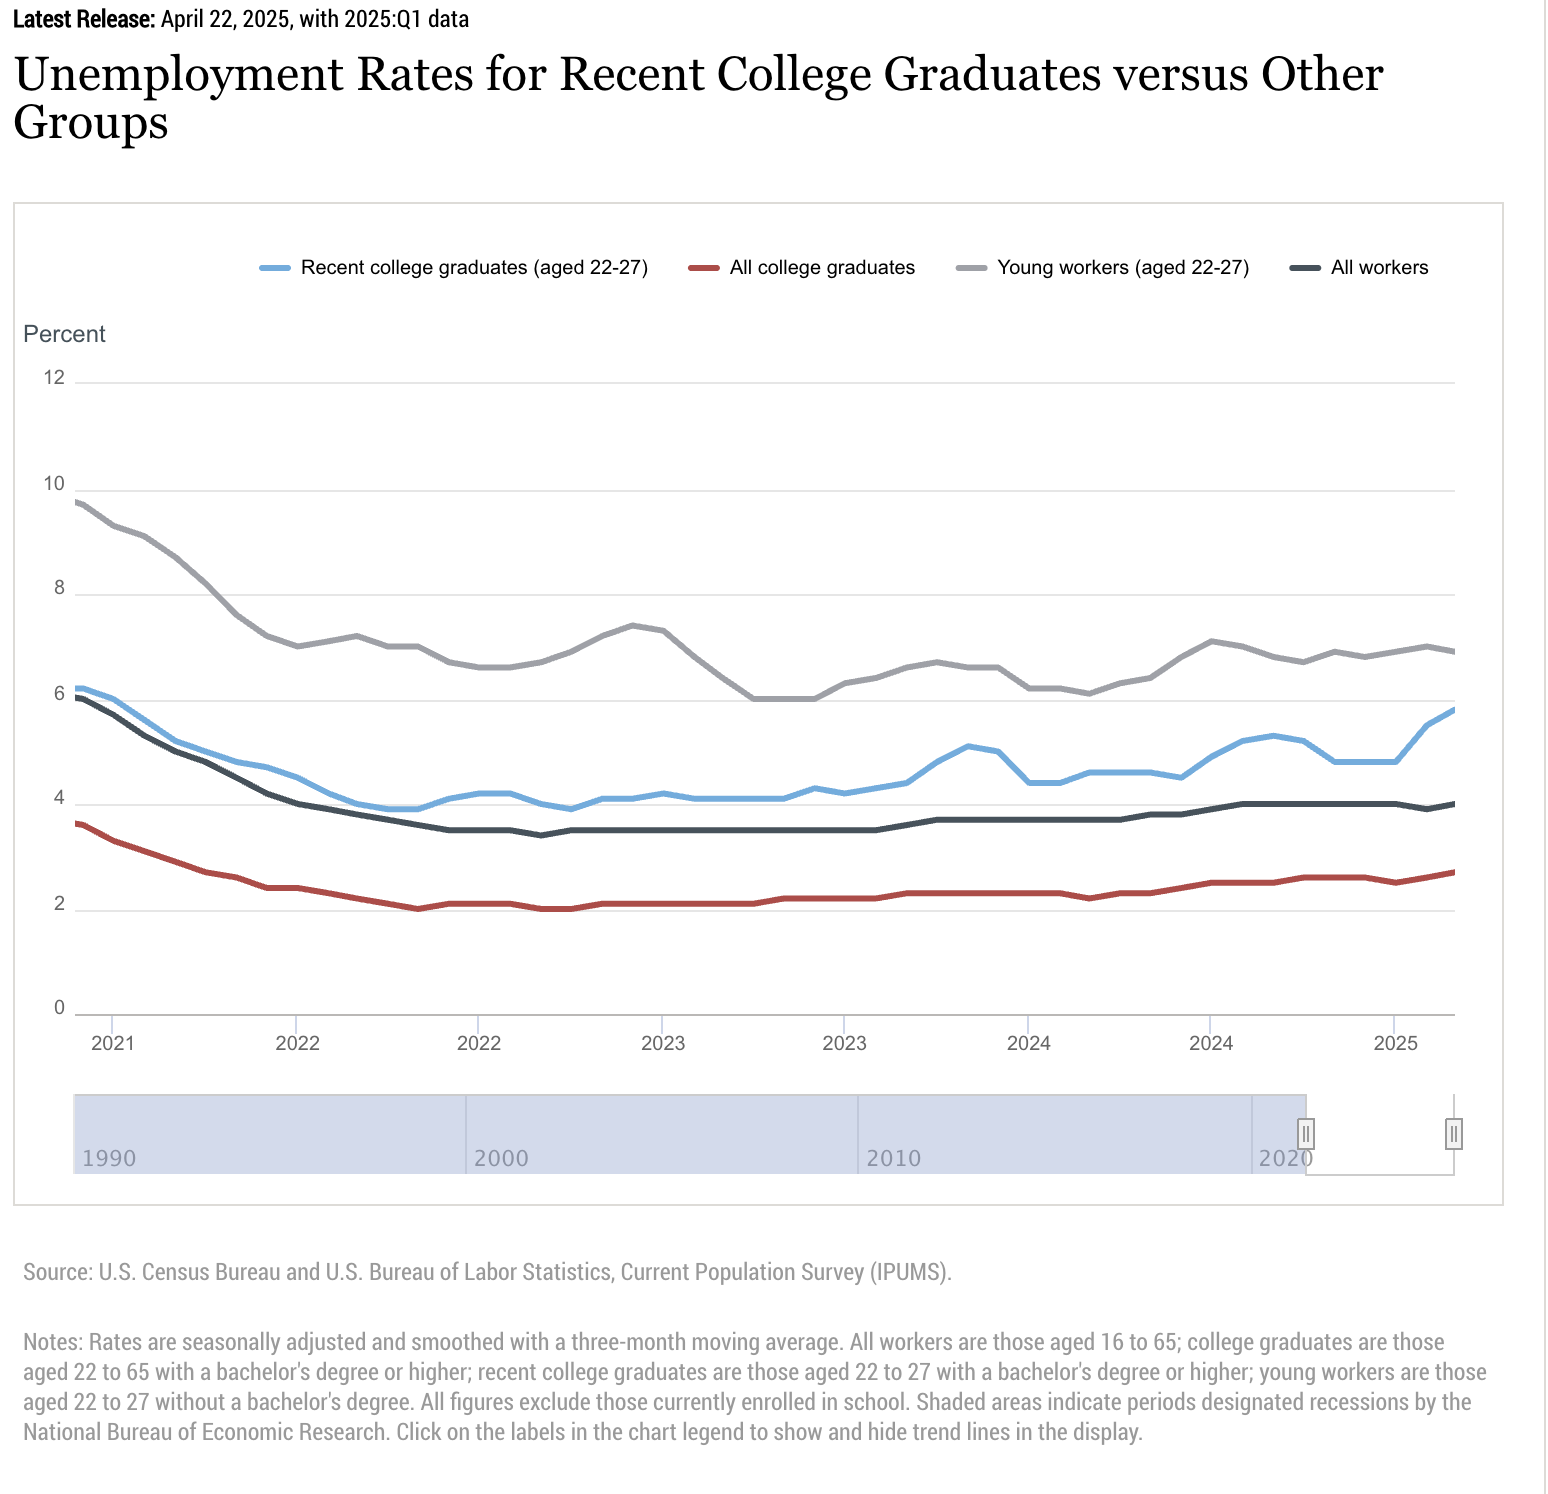
\includegraphics[keepaspectratio]{images/unemployment_rate_recent_graduate.png}}

}

\caption{\label{fig-graduates}Unemployment Rate of Recent College
Graduates}

\end{figure}%

Although the Federal Open Market Committee (FOMC) reported a low overall
unemployment rate for June 2025 (Based on the U.S. Bureau of Labor
Statistics (BLS) revised job creation data released on July 31, 2025, a
marked decline in job creation has been observed beginning in May,
raising substantial concerns regarding the stability of the U.S. labor
market.), recent data clearly indicate a noticeable uptick in the
unemployment rate for the 22-27 age group since March, reaching 2021
levels and particularly affecting recent college graduates
(Figure~\ref{fig-graduates}).

\section{Data}\label{data}

\textsubscript{Source:
\href{https://mw1296.github.io/dsan5650_social_causal_inference/index.qmd.html}{Article
Notebook}}

\begin{longtable}[]{@{}llll@{}}

\caption{\label{tbl-monthly-unemployment-rate-race}BLS 2015-2025 Monthly
Unemployment Rate By Race}

\tabularnewline

\caption{}\label{T_bcf33}\tabularnewline
\toprule\noalign{}
Year & Month & Unemployment\_rate & Race \\
\midrule\noalign{}
\endfirsthead
\toprule\noalign{}
Year & Month & Unemployment\_rate & Race \\
\midrule\noalign{}
\endhead
\bottomrule\noalign{}
\endlastfoot
2015 & Jan & 5.30 & white \\
2016 & Jan & 4.70 & white \\
2017 & Jan & 4.70 & white \\
2018 & Jan & 3.90 & white \\
2019 & Jan & 4.00 & white \\
2020 & Jan & 3.50 & white \\
2021 & Jan & 6.20 & white \\
2022 & Jan & 3.90 & white \\
2023 & Jan & 3.50 & white \\
2024 & Jan & 3.80 & white \\

\end{longtable}

\textsubscript{Source:
\href{https://mw1296.github.io/dsan5650_social_causal_inference/index.qmd.html}{Article
Notebook}}

Data from the U.S. Bureau of Labor Statistics (BLS) 2015 to 2025 monthly
aggregated unemployment rate by races. This dataset is used to analyze
the race effect on unemployment along with the monthly unemployment rate
aggregated data by race
(Table~\ref{tbl-monthly-unemployment-rate-race}).

\textsubscript{Source:
\href{https://mw1296.github.io/dsan5650_social_causal_inference/index.qmd.html}{Article
Notebook}}

\textsubscript{Source:
\href{https://mw1296.github.io/dsan5650_social_causal_inference/index.qmd.html}{Article
Notebook}}

\begin{longtable}[]{@{}llllllll@{}}

\caption{\label{tbl-survey-data-jun2025}BLS June 2025 Labor Force Survey
Data}

\tabularnewline

\caption{}\label{T_51442}\tabularnewline
\toprule\noalign{}
sex\_name & race\_name & education\_attainment\_name &
employment\_status\_name & industry\_name & is\_black\_african &
is\_asian & is\_white \\
\midrule\noalign{}
\endfirsthead
\toprule\noalign{}
sex\_name & race\_name & education\_attainment\_name &
employment\_status\_name & industry\_name & is\_black\_african &
is\_asian & is\_white \\
\midrule\noalign{}
\endhead
\bottomrule\noalign{}
\endlastfoot
male & white & bachelors\_degree & employed & Construction & 0 & 0 &
1 \\
male & white & high\_school & employed & Construction & 0 & 0 & 1 \\
female & white & bachelors\_degree & employed & Manufacturing & 0 & 0 &
1 \\
male & white & bachelors\_degree & employed & Manufacturing & 0 & 0 &
1 \\
female & white & masters\_degree & employed & Transportation and
utilities & 0 & 0 & 1 \\
female & white & bachelors\_degree & employed & Construction & 0 & 0 &
1 \\
male & white & high\_school & employed & Wholesale and retail trade & 0
& 0 & 1 \\
female & white & bachelors\_degree & employed & Professional and
business services & 0 & 0 & 1 \\
male & white & less\_than\_high\_school & employed & Professional and
business services & 0 & 0 & 1 \\
female & white & high\_school & employed & Educational and health
services & 0 & 0 & 1 \\

\end{longtable}

\textsubscript{Source:
\href{https://mw1296.github.io/dsan5650_social_causal_inference/index.qmd.html}{Article
Notebook}}

Data from the U.S. Bureau of Labor Statistics (BLS) June 2025 labor
force survey provide individual-level employment status and
corresponding demographic information. For the purpose of this study, a
subset of these relevant columns is utilized
(Table~\ref{tbl-survey-data-jun2025}). This dataset is used to sample
and predict employment status using the observations in the survey data.

\textsubscript{Source:
\href{https://mw1296.github.io/dsan5650_social_causal_inference/index.qmd.html}{Article
Notebook}}

\begin{longtable}[]{@{}lllll@{}}

\caption{\label{tbl-survey-data-2024-2025}BLS 2024 - 2025 Jan - Jul
Labor Force Survey Data}

\tabularnewline

\caption{}\label{T_cc2f2}\tabularnewline
\toprule\noalign{}
industry & employment\_status & month\_year & industry\_name &
employment\_status\_description \\
\midrule\noalign{}
\endfirsthead
\toprule\noalign{}
industry & employment\_status & month\_year & industry\_name &
employment\_status\_description \\
\midrule\noalign{}
\endhead
\bottomrule\noalign{}
\endlastfoot
11 & 1 & jan\_2024 & Leisure and hospitality & employed \\
11 & 1 & jan\_2024 & Leisure and hospitality & employed \\
10 & 1 & jan\_2024 & Educational and health services & employed \\
5 & 1 & jan\_2024 & Wholesale and retail trade & employed \\
4 & 4 & jan\_2024 & Manufacturing & unemployed \\
8 & 1 & jan\_2024 & Financial activities & employed \\
9 & 1 & jan\_2024 & Professional and business services & employed \\
5 & 1 & jan\_2024 & Wholesale and retail trade & employed \\
4 & 1 & jan\_2024 & Manufacturing & employed \\
4 & 1 & jan\_2024 & Manufacturing & employed \\

\end{longtable}

\textsubscript{Source:
\href{https://mw1296.github.io/dsan5650_social_causal_inference/index.qmd.html}{Article
Notebook}}

Data from the U.S. Bureau of Labor Statistics (BLS) historical monthly
labor force survey provide individual-level employment status by
industries. For the purpose of this study, we utilized 2024 Jan to Jul
and 2025 Jan to Jun data. (Table~\ref{tbl-survey-data-2024-2025}). This
dataset is used to analyze the industry effect on unemployment rate in
the recent 2 years.

\section{EDA}\label{eda}

\subsection{Unemployment Rates of Differenet
Races}\label{unemployment-rates-of-differenet-races}

\textsubscript{Source:
\href{https://mw1296.github.io/dsan5650_social_causal_inference/index.qmd.html}{Article
Notebook}}

\begin{verbatim}
Unemployment Rate Distribution Histograms By Race
\end{verbatim}

\pandocbounded{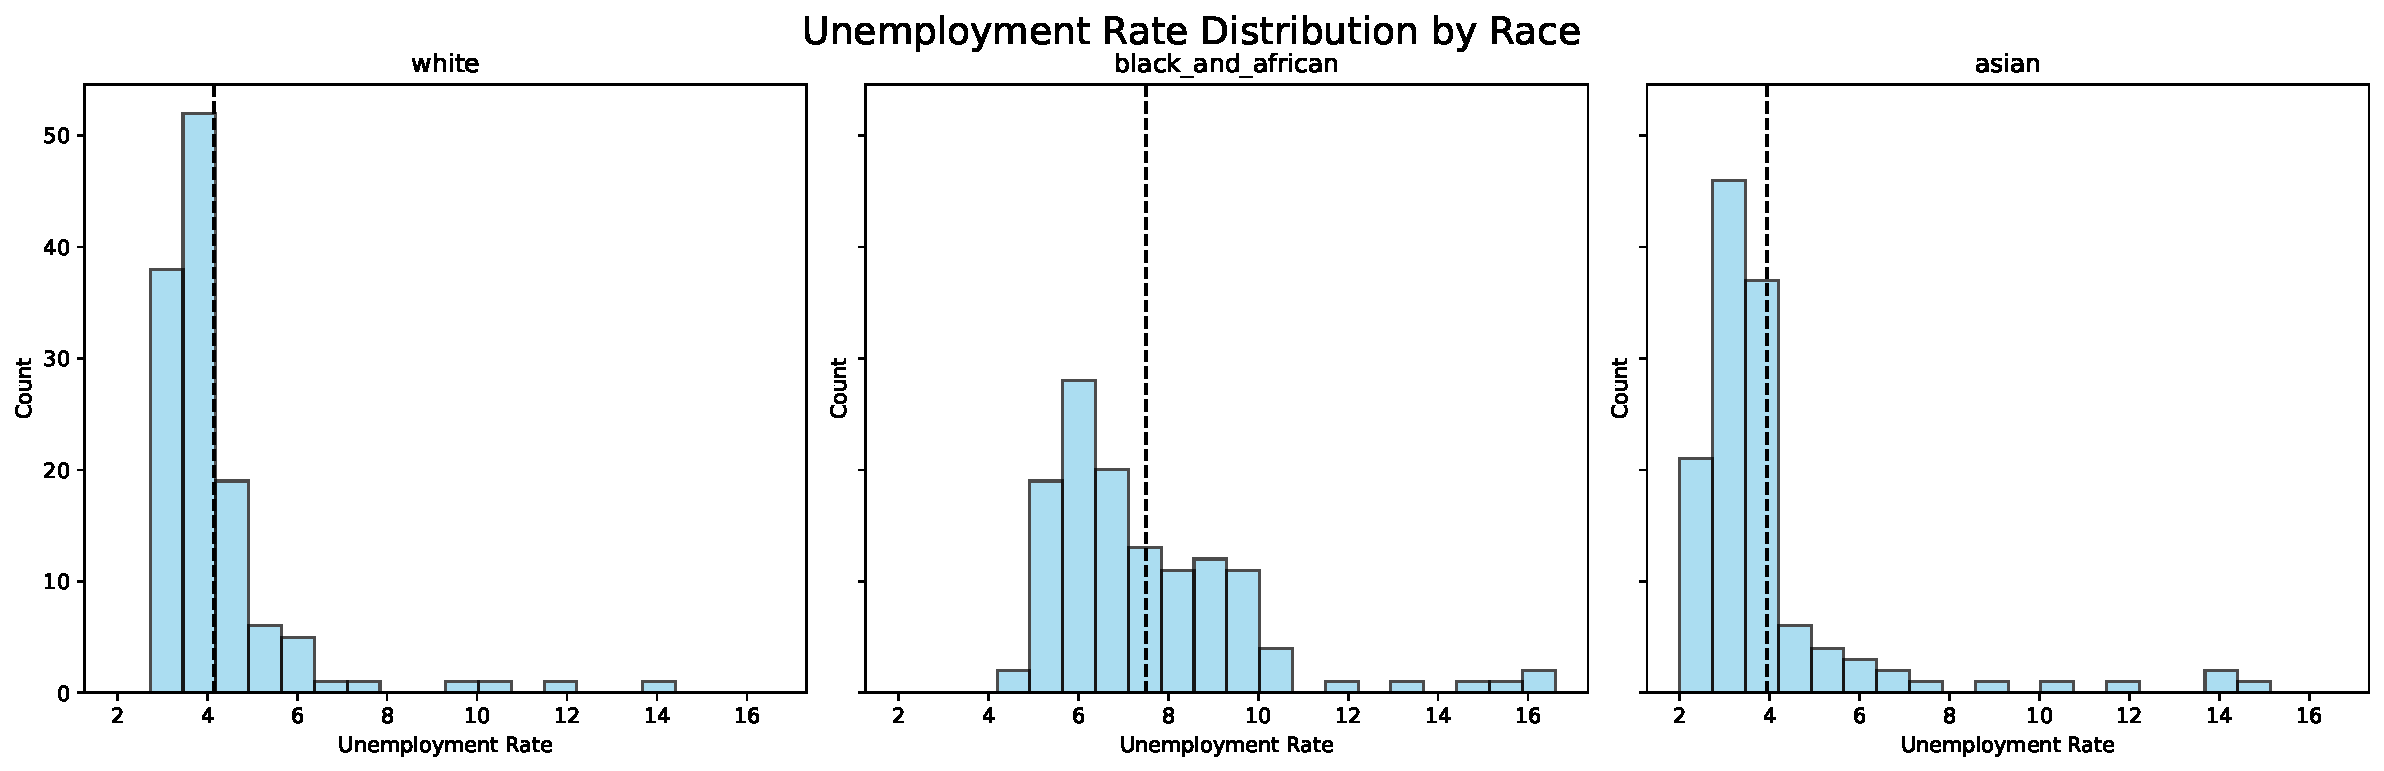
\includegraphics[keepaspectratio]{index_files/figure-pdf/cell-7-output-2.pdf}}

\begin{verbatim}
Unemployment Rate Distribution Histograms By Sex
\end{verbatim}

\pandocbounded{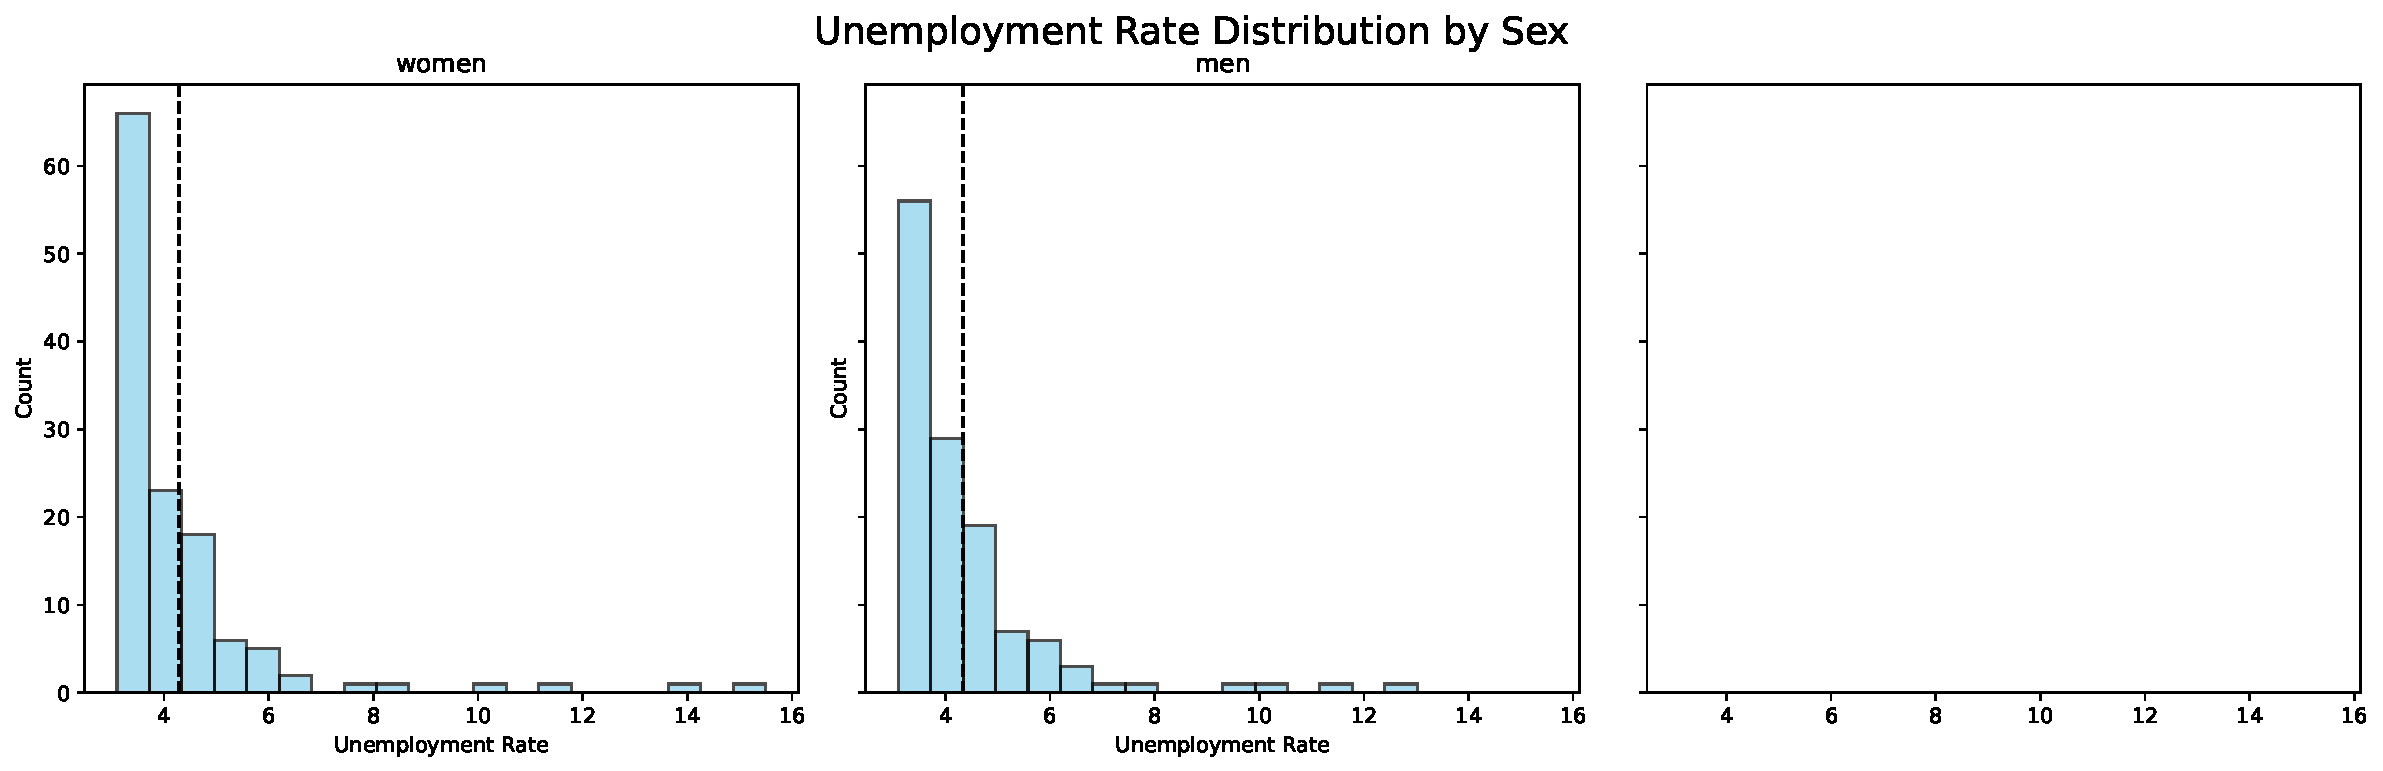
\includegraphics[keepaspectratio]{index_files/figure-pdf/cell-7-output-4.pdf}}

\begin{verbatim}
Unemployment Rate Distribution Histograms By Industry
\end{verbatim}

\pandocbounded{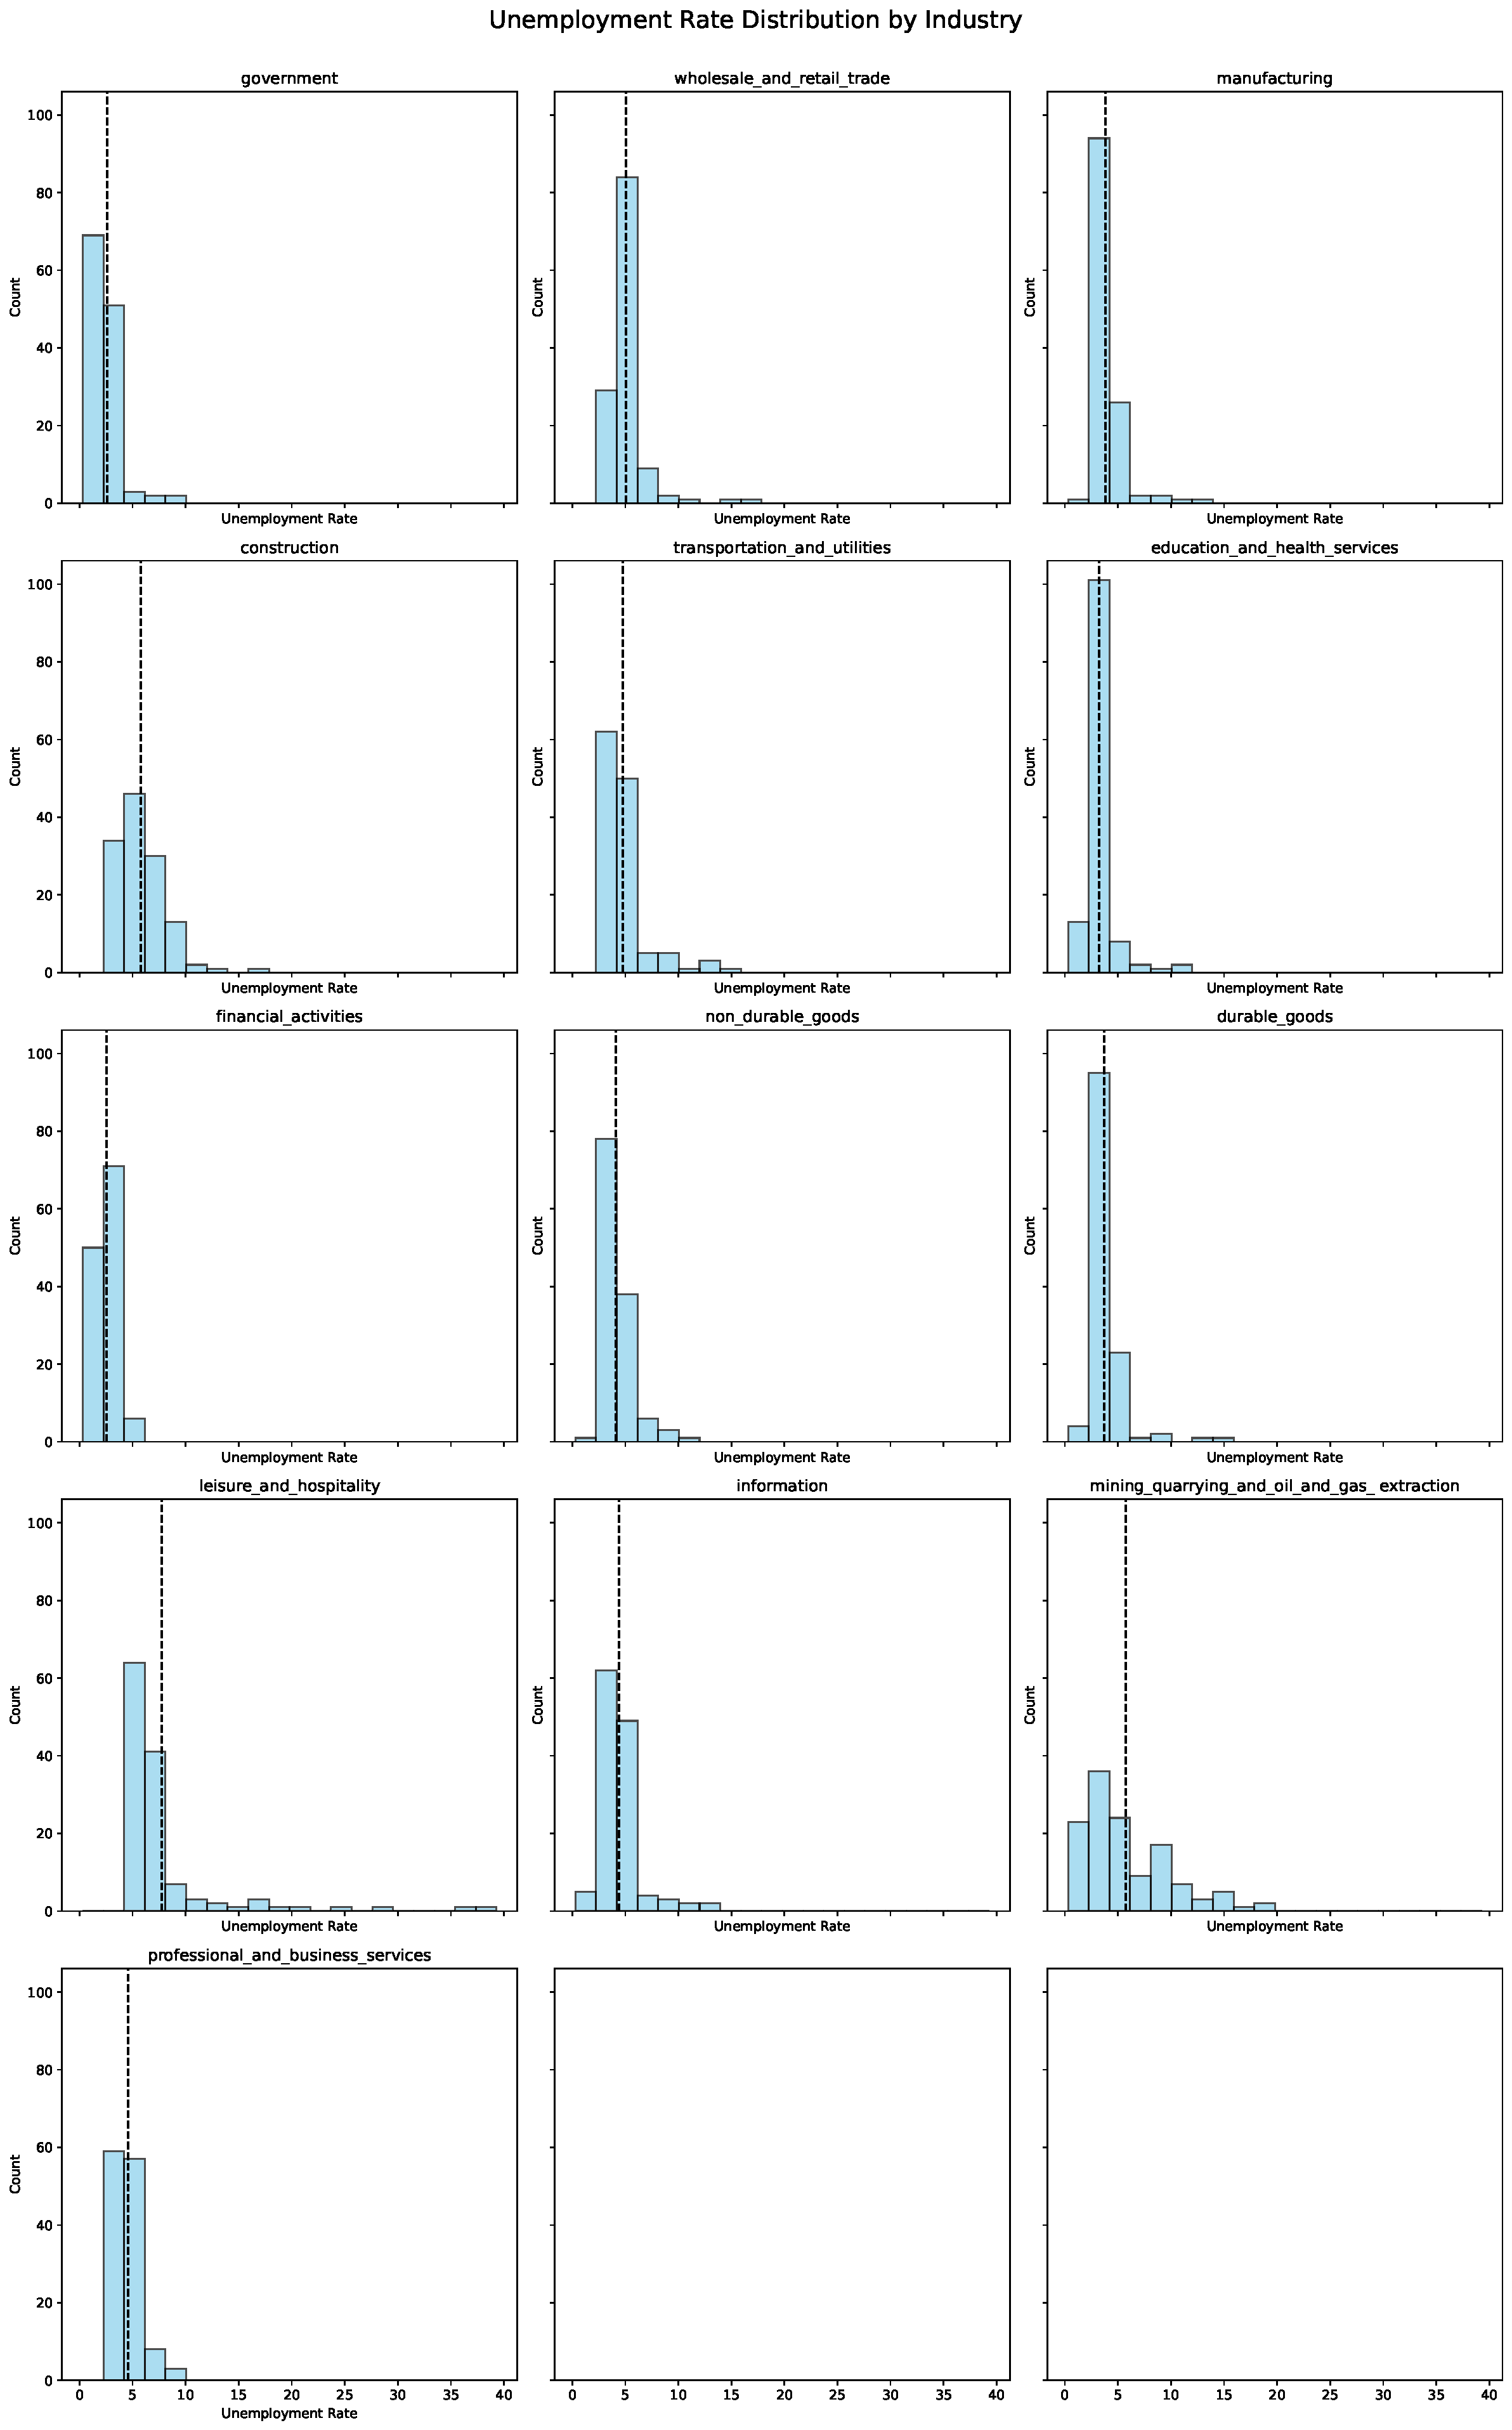
\includegraphics[keepaspectratio]{index_files/figure-pdf/cell-7-output-6.pdf}}

\begin{verbatim}
Unemployment Rate Distribution Histograms By Age
\end{verbatim}

\pandocbounded{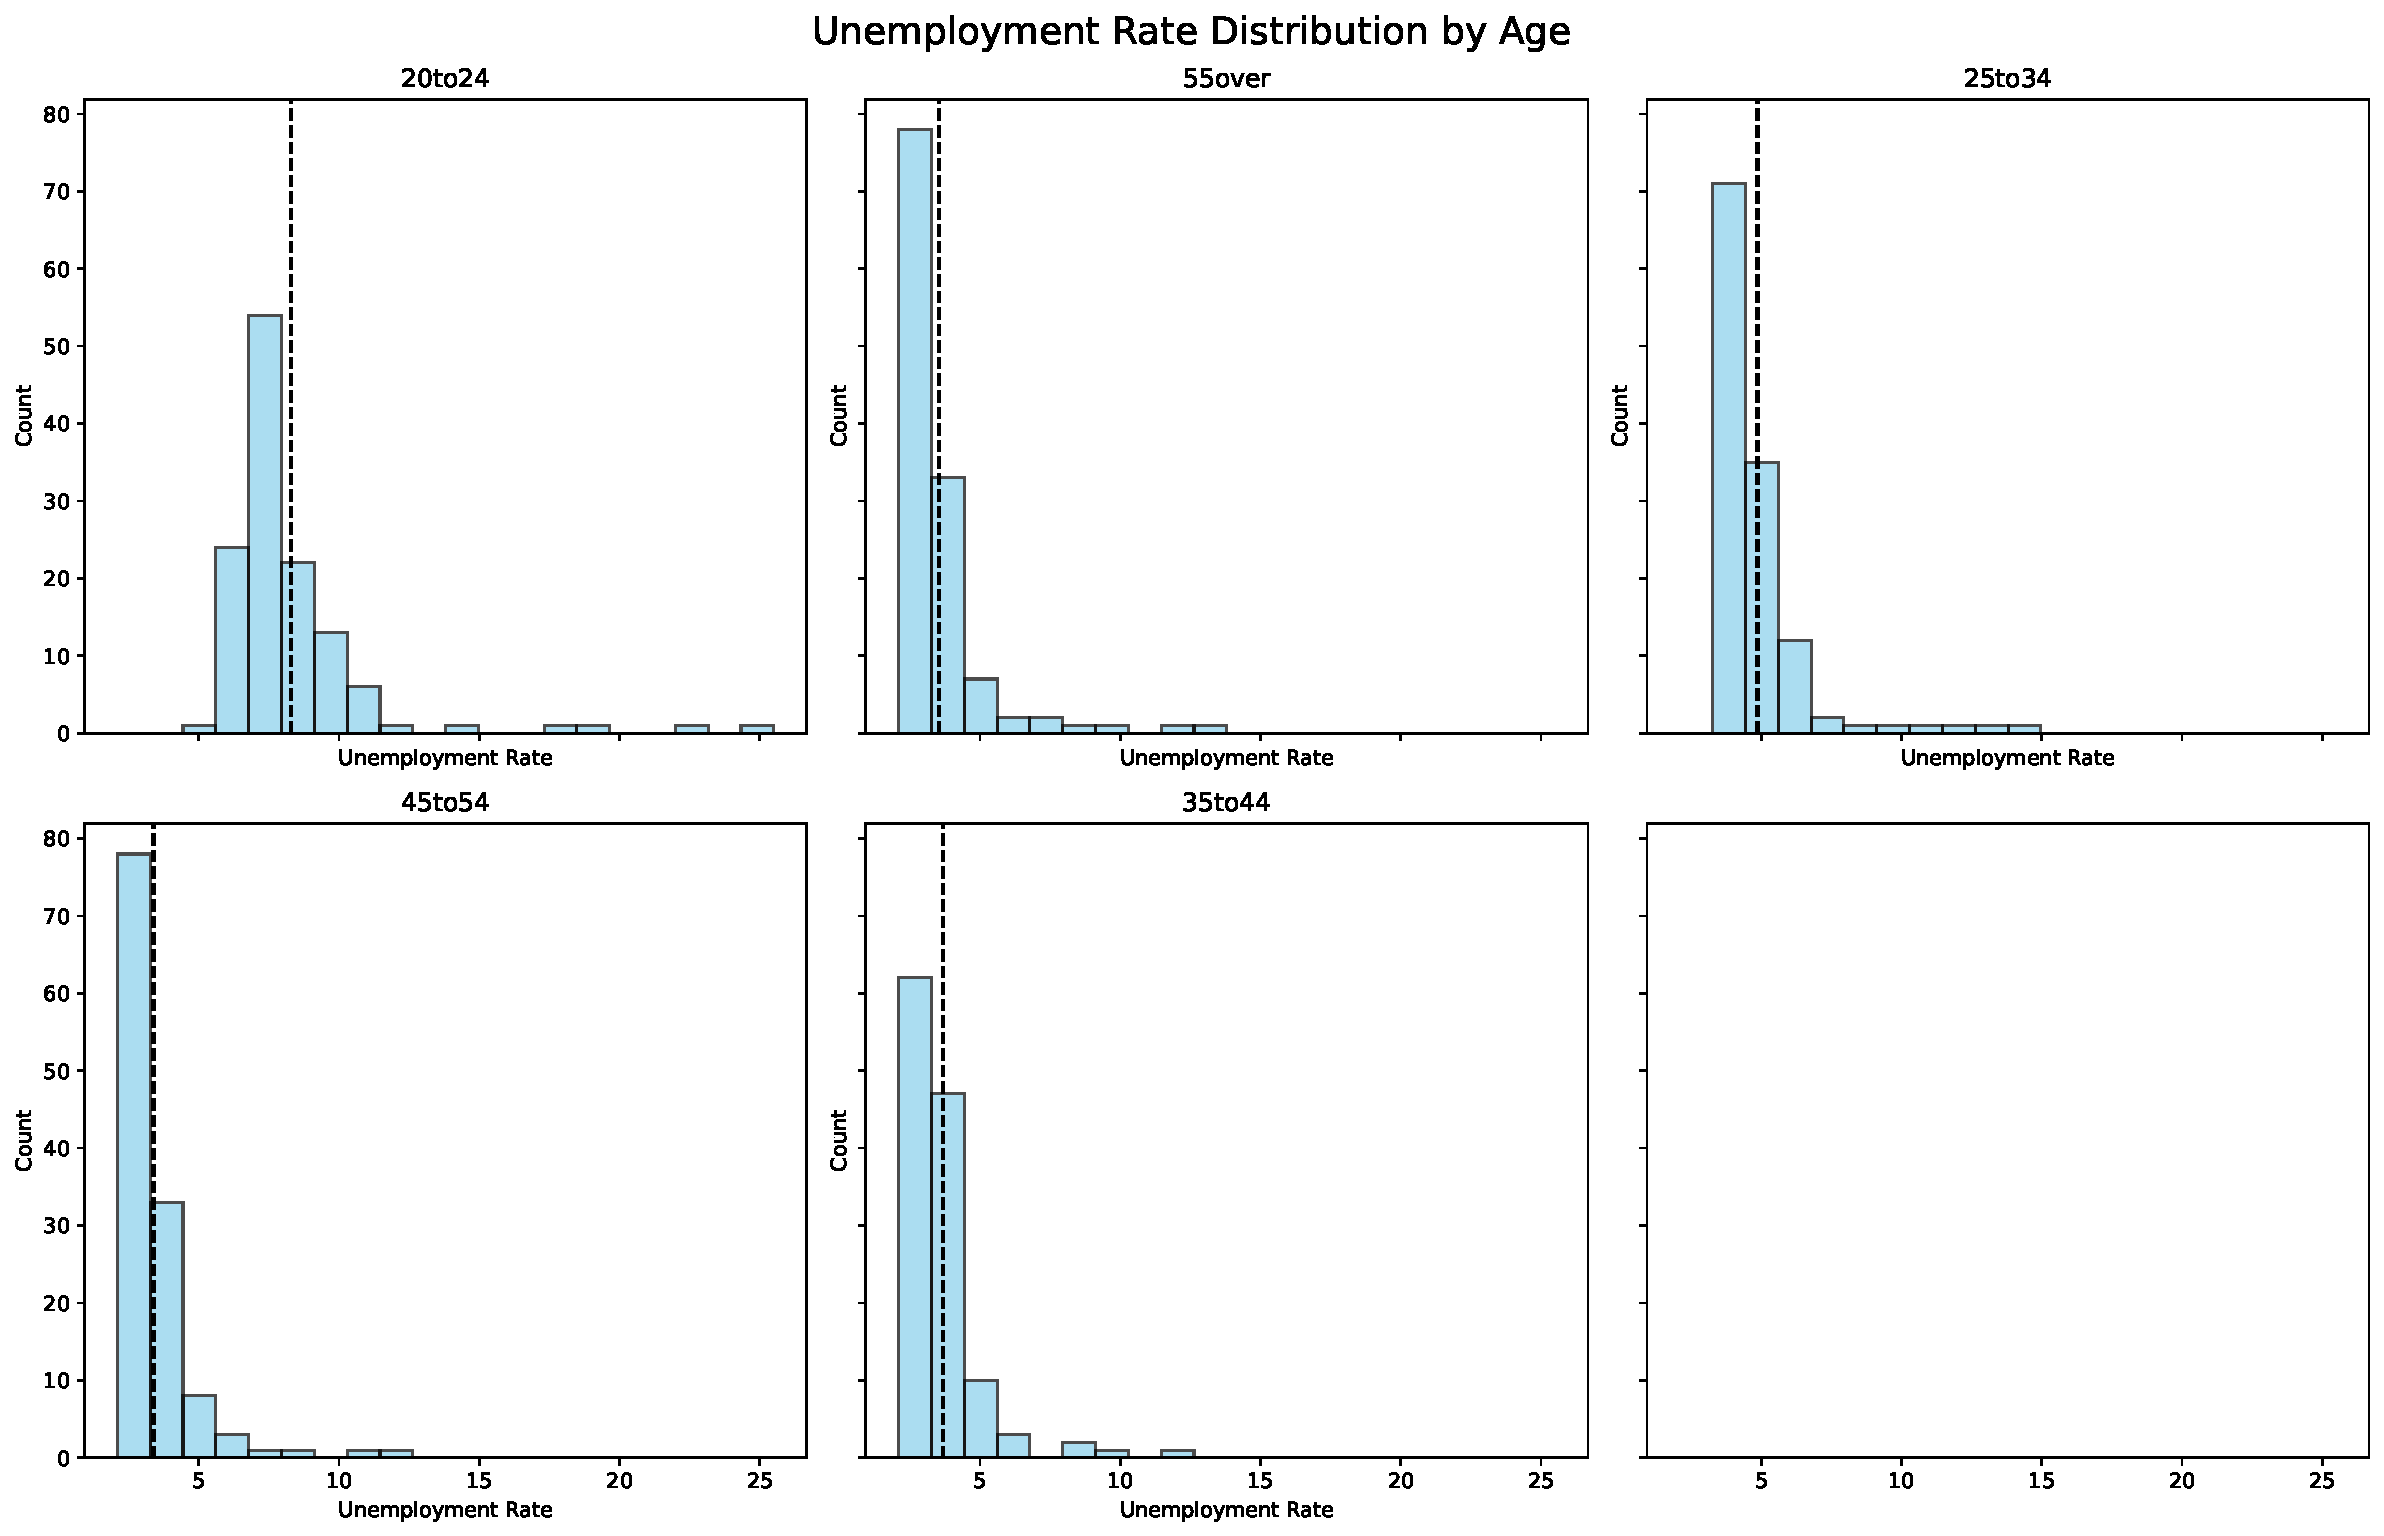
\includegraphics[keepaspectratio]{index_files/figure-pdf/cell-7-output-8.pdf}}

\textsubscript{Source:
\href{https://mw1296.github.io/dsan5650_social_causal_inference/index.qmd.html}{Article
Notebook}}

\begin{verbatim}
Unemployment Rate Distribution Histograms By Education_attainment
\end{verbatim}

\begin{figure}[H]

\centering{

\pandocbounded{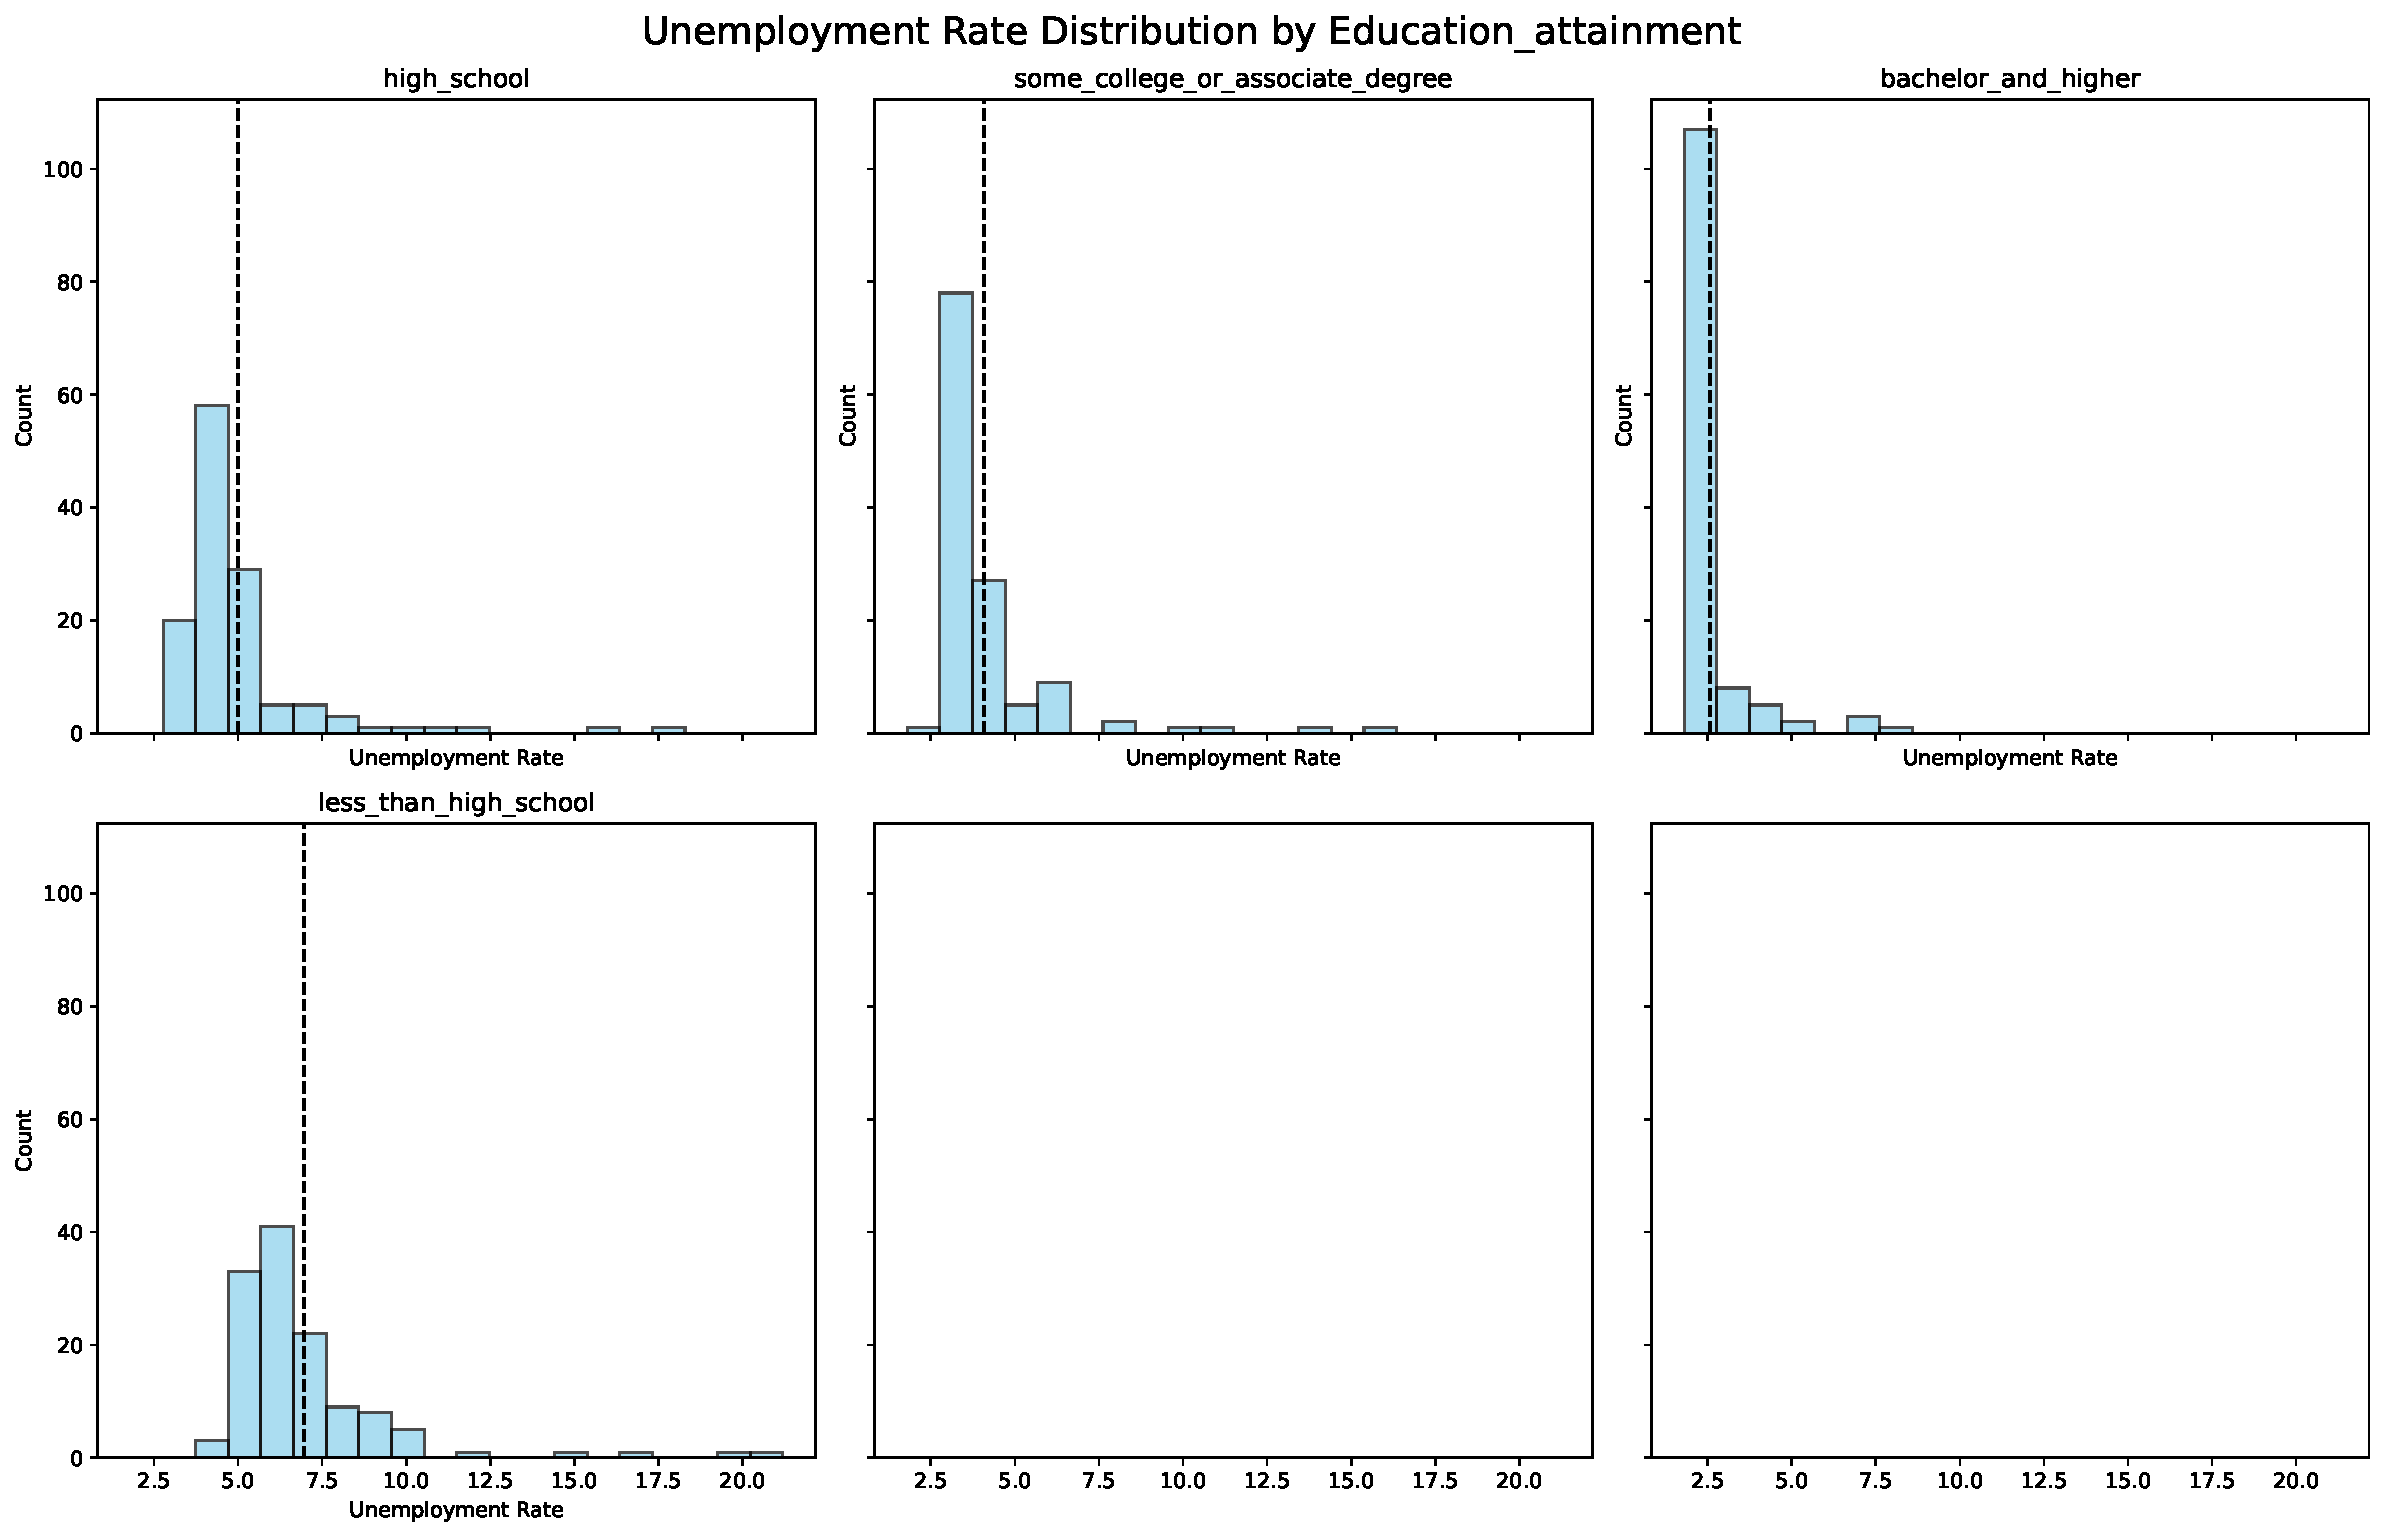
\includegraphics[keepaspectratio]{index_files/figure-pdf/fig-histogram-unemployment-rate-demographics-output-2.pdf}}

}

\caption{\label{fig-histogram-unemployment-rate-demographics}Unemployment
Rate Distributions By Demographics (2015-2025 statistics)}

\end{figure}%

\textsubscript{Source:
\href{https://mw1296.github.io/dsan5650_social_causal_inference/index.qmd.html}{Article
Notebook}}

BLS data from 2015--2025 indicate that the Black or African American
population experienced the highest average unemployment rate (7.5\%),
primarily within the 5--10\% range. Gender differences are minimal, with
both averaging around 5\%, though rates are slightly higher for men.
Among industries, Leisure and Hospitality recorded the highest
unemployment (10\%) with a long-tail distribution, followed by
Agriculture (5--11\%) and moderate variability. Construction and
Mining/Oil \& Gas exhibit similar but marginally lower patterns. The
22--24 age group stands out with significantly elevated
unemployment---averaging 7\% and predominantly above 5\%---while other
age groups display lower and more uniform rates. Financial Activities
show the lowest and most stable unemployment, consistently under 5\%.
Individuals without a high school diploma face high and variable
unemployment, averaging 7\% with a long-tail skew. These patterns
suggest that young adults (22--24), Black or African Americans without
college degrees, and those employed in Leisure, Construction, or Mining
sectors are disproportionately affected by higher unemployment.
(Figure~\ref{fig-histogram-unemployment-rate-demographics}).

\textsubscript{Source:
\href{https://mw1296.github.io/dsan5650_social_causal_inference/index.qmd.html}{Article
Notebook}}

\begin{figure}[H]

\centering{

\pandocbounded{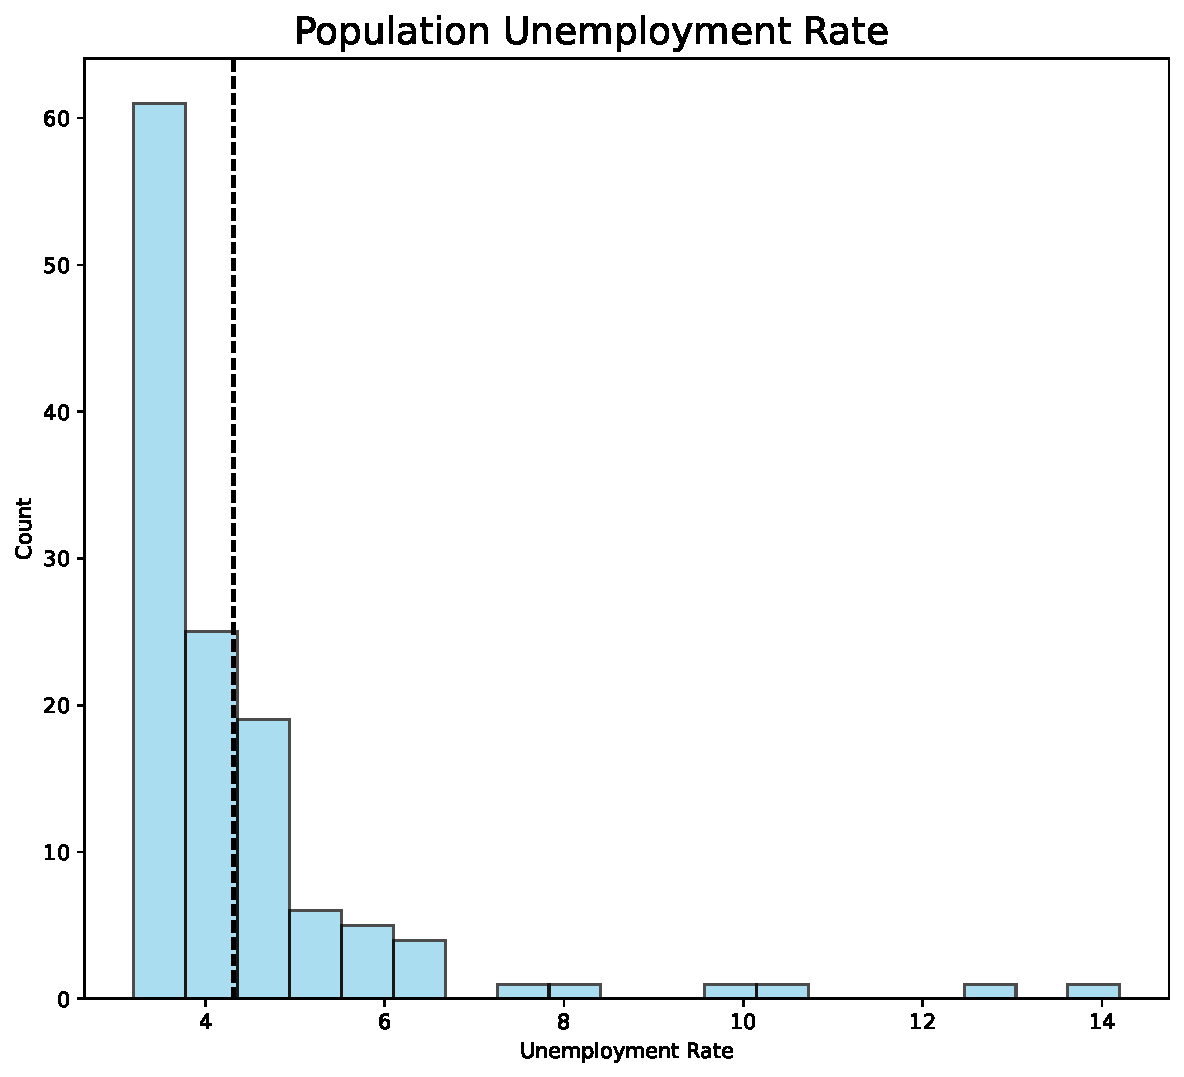
\includegraphics[keepaspectratio]{index_files/figure-pdf/fig-histogram-unemployment-rate-output-1.pdf}}

}

\caption{\label{fig-histogram-unemployment-rate}Overall Population
Unemployment Rate Distributions (2015-2025 statistics)}

\end{figure}%

\textsubscript{Source:
\href{https://mw1296.github.io/dsan5650_social_causal_inference/index.qmd.html}{Article
Notebook}}

According to BLS data from 2015--2025, the overall population
unemployment rate averaged slightly above 4\%, with the majority of
observations concentrated between 2\% and 5\% and exhibiting relatively
low variability (Figure~\ref{fig-histogram-unemployment-rate}).

\subsection{Unemployment Rates of Differenet
Industries}\label{unemployment-rates-of-differenet-industries}

\textsubscript{Source:
\href{https://mw1296.github.io/dsan5650_social_causal_inference/index.qmd.html}{Article
Notebook}}

\begin{figure}[H]

\centering{

\pandocbounded{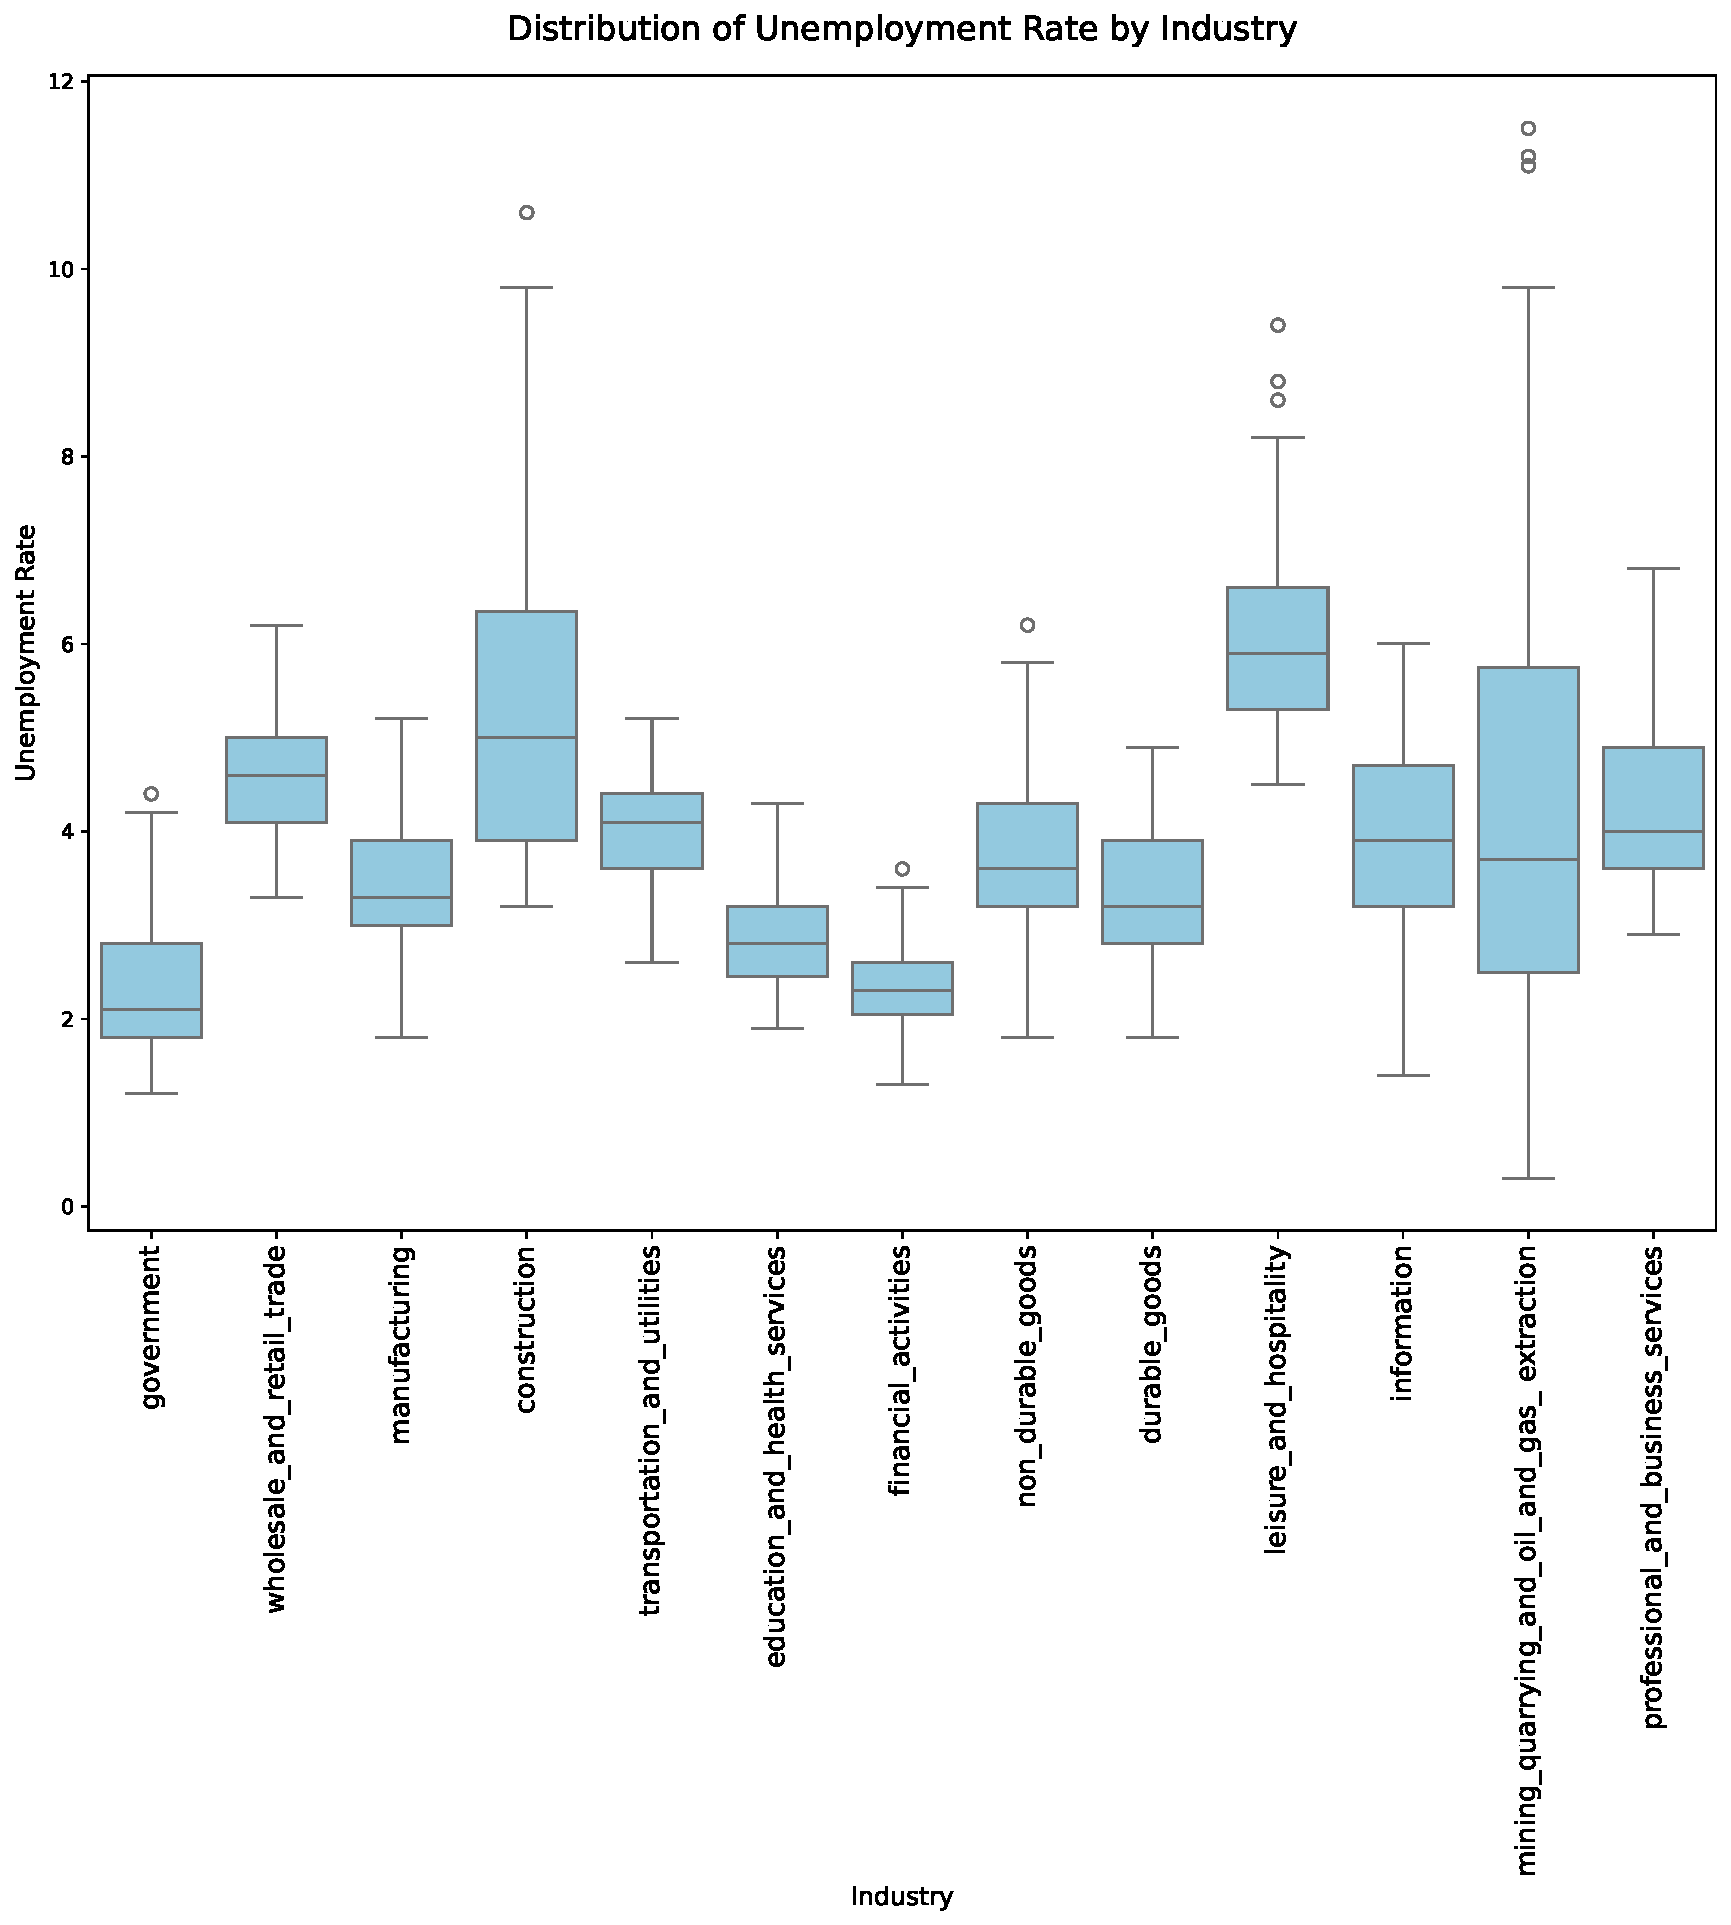
\includegraphics[keepaspectratio]{index_files/figure-pdf/fig-boxplot-unemployment-rate-industry-output-1.pdf}}

}

\caption{\label{fig-boxplot-unemployment-rate-industry}Unemployment Rate
Distributions By Industries (2015-2025 statistics)}

\end{figure}%

\textsubscript{Source:
\href{https://mw1296.github.io/dsan5650_social_causal_inference/index.qmd.html}{Article
Notebook}}

The boxplot illustrates notable variation in unemployment rates across
industries. ``Agricultural, mining/oil/gas extraction'' and
``Construction'' industries exhibit the highest variation and upper
extremes, indicating greater instability in employment. Due to the
volatility and unpredictivity as a result of seasonlity, these two
categories are going to be excluded from our analysis. In contrast,
``Government'', ``Financial services'', and ``Education/health
services'' show consistently low and stable unemployment rates, with
narrower interquartile ranges and fewer outliers. These patterns suggest
structural differences in labor market vulnerability across sectors.
(Figure~\ref{fig-boxplot-unemployment-rate-industry}).

\section{PGM}\label{pgm}

We posit that unemployment vulnerability is driven by structural
inequalities within the labor market, particularly those rooted in
demographic and industrial dimensions. Demographic disparities are
represented by variables such as race, age, and educational attainment
and industry; sex is excluded from the analysis due to prior findings
indicating minimal impact on unemployment rates. Establishing a baseline
unemployment level is a necessary step before assessing the marginal
effects of these demographic and industrial factors.

\subsection{Baseline unemployment rate
distribution}\label{baseline-unemployment-rate-distribution}

Figure 3 illustrates that the population unemployment rate is
right-skewed, suggesting that the Log-Normal distribution is an
appropriate model. We are going to estimate the parameters of a
Log-Normal distribution from the population distribution data using MLE.
(\(\sigma\), \(\text{loc}\), and \(\text{scale}\)).

\textsubscript{Source:
\href{https://mw1296.github.io/dsan5650_social_causal_inference/index.qmd.html}{Article
Notebook}}

\begin{verbatim}

Fitted Log-Norm Distribution Parameters:
  Shape parameter 'alpha'): 9.92
  Location parameter (loc): 3.20
  Scale parameter (scale): 0.03
\end{verbatim}

\begin{figure}[H]

\centering{

\pandocbounded{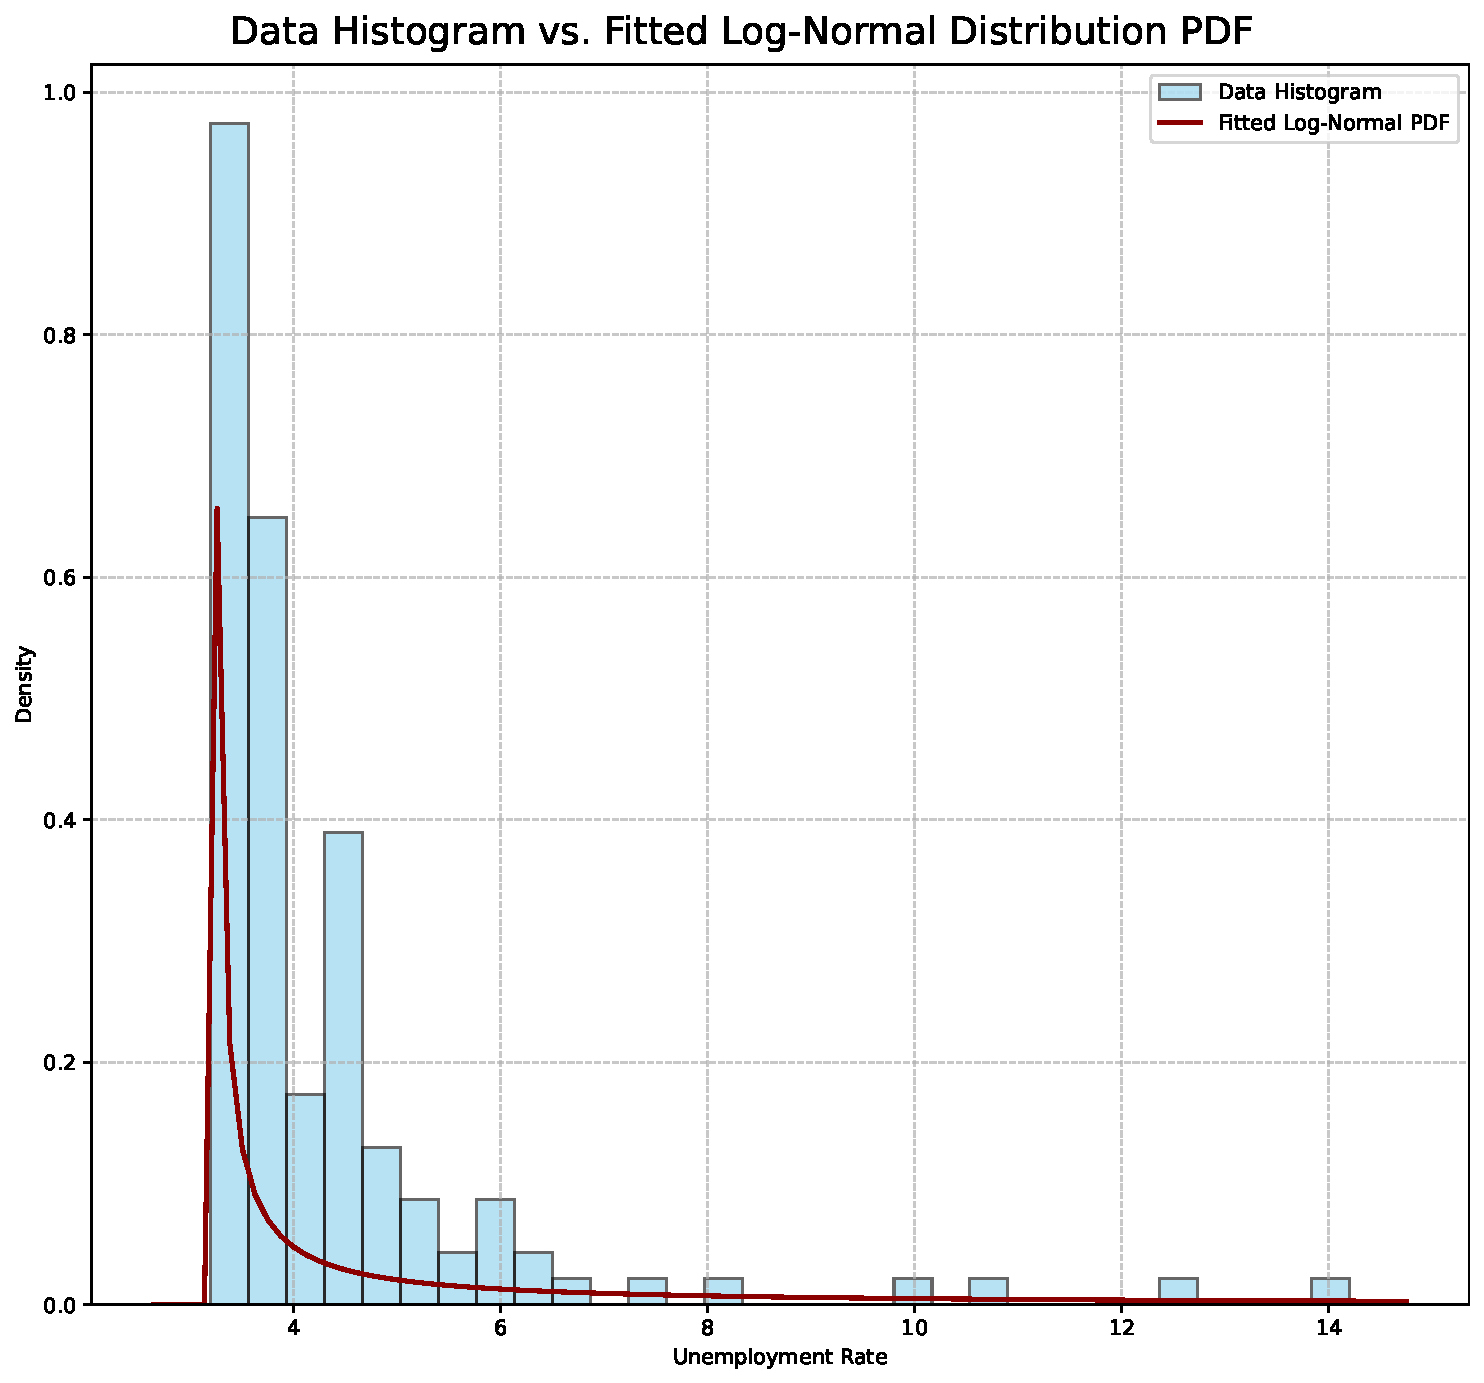
\includegraphics[keepaspectratio]{index_files/figure-pdf/fig-histogram-lognorm-output-2.pdf}}

}

\caption{\label{fig-histogram-lognorm}Unmployment Rate Histogram
vs.~Fitted Log-Norm PDF}

\end{figure}%

\textsubscript{Source:
\href{https://mw1296.github.io/dsan5650_social_causal_inference/index.qmd.html}{Article
Notebook}}

By overlaying the smooth PDF curve on top of original data's histogram,
we can visualize that the Log-Normal distribution matches the
distribution of the actual data. The peak of the PDF align with the peak
of the histogram. The spread of the PDF roughly match the spread of the
data, including the tail (Figure~\ref{fig-histogram-lognorm}). Now we
need to use Kolmogorov-Smirnov Test to test Goodness-of-fit with the
original data and estimated parameters, then examine the p value.

\section*{References}\label{references}
\addcontentsline{toc}{section}{References}

\vspace{1em}

\textsubscript{Source:
\href{https://mw1296.github.io/dsan5650_social_causal_inference/index.qmd.html}{Article
Notebook}}

\phantomsection\label{refs}
\begin{CSLReferences}{1}{0}
\bibitem[\citeproctext]{ref-Joseph2024}
Joseph Dean, E. S. (2024). \href{}{Gender differences in unemployment
trends: Race, jobs and the economy update for february 2024}.
\emph{NCRC}.

\bibitem[\citeproctext]{ref-TOIEducation2025}
TOIEducation. (2025). \href{}{Degrees at risk: 10 US college majors with
the highest unemployment rate in 2025}. \emph{The Times Of India}.

\bibitem[\citeproctext]{ref-Oberlo2024}
\href{}{US UNEMPLOYMENT RATE BY INDUSTRY (2024)}. (2024). \emph{Oberlo}.

\bibitem[\citeproctext]{ref-ValerieWilson2022}
Wilson, V., \& Darity-Jr., W. (2022). \href{}{Understanding black-white
disparities in labor market outcomes requires models that account for
persistent discrimination and unequal bargaining power}. \emph{Economic
Policy Institute}.

\bibitem[\citeproctext]{ref-YiLiChienandPaulMorris}
YiLi Chien, P. M. (2016). \href{}{Unemployment by industry: Duration
must be considered, too}. \emph{Federal Reserve Bank of St.Lois -
Regional Economist}.

\end{CSLReferences}




\end{document}
